\chapter{Zusätzliche Funktionen der App}
\label{chap:6}

Zu den in \autoref{chap:1} vorgestellten Funktionen wurden noch zusätzliche Funktionen implementiert, welche die Nutzung der App erleichtern sollen.

Zuerst wurde eine Navigation über Tabs umgesetzt, mit welcher der Nutzer immer zwischen der Karte und der Liste wechseln kann. Hierfür wurde wieder das React Navigation Paket \cite{reactNavigation} verwendet. Die Komponente für die Tab-Navigation trägt den Namen material-top-tabs, da diese Tabs oben am Bildschirm angesiedelt sind. Wie in \autoref{fig:details1} zu sehen ist, werden die Tabs auch bei Öffnen eines Detail-Fensters beibehalten, sodass immer eine Navigation zur Karte möglich ist. Damit kann der Nutzer Daten eines bestimmten Parkhauses nachschauen und kann dieses Parkhaus auch auf der Karte betrachten, ohne, dass immer ein Fenster geschlossen werden müsste, um zurück zur Karte navigieren zu können. Die Umsetzung der Tabs ist in der Datei \verb|App.tsx| zu finden.

Eine weitere Funktion ist die Navigation zu einem bestimmten Parkhaus von überall in der App. Es kann sowohl von der Karte, als auch von den Detail-Fenstern der Parkhäuser immer zu dem gewünschten Parkhaus navigiert werden. Auch wird durch die \verb|findCorrectGpxFile|-Funktion sichergestellt, dass die Weiterleitung zu Google Maps immer in der Komponente stattfindet, in welcher der Navigations-Knopf gedrückt wurde. Zum Beispiel wird bei Drücken des Knopfes zur Navigation in einem Detail-Fenster nicht zur Karte navigiert und dann weitergeleitet, sondern das Detail-Fenster bleibt offen und die Weiterleitung findet hier statt. Somit bleibt die App genau in dem Zustand, in welchem der Nutzer diese zur Navigation mit Google Maps verlässt und es kommt zu keinen Brüchen in der Nutzererfahrung.

Für die letzte zusätzliche Funktion wird die in \autoref{chap:5} beschriebene Navigation zum nähesten Parkhaus benötigt. Diese Funktion ist durch den Knopf mit der Aufschrift ,,Starten'', welcher in \autoref{fig:map} rechts unten ersichtlich ist, umgesetzt. Ein Drücken dieses Knopfes kann zwei Effekte haben. Wenn der Nutzer sich in keinem der Geofences der neun Parkhäuser befindet, wird automatisch zum nähesten Parkhaus weitergeleitet. Dafür wird wieder die \verb|findCorrectGpxFile|-Funktion benutzt, welche, wie in \autoref{chap:5} beschrieben, die Startpunkte der GPX-Dateien mit der Position des Nutzers vergleicht. Die GPX-Datei mit dem nähesten Startpunkt wird verwendet. Da alle GPX-Dateien immer zum nähesten Parkhaus von ihrem Startpunkt aus führen, wird somit immer zum nähesten Parkhaus navigiert. Dies funktioniert jedoch nur, wenn der Nutzer sich auf dem Altstadtring befindet. Wenn nicht, also wenn die Entfernung zwischen Nutzer und allen Startpunkten der GPX-Dateien mehr als 100 Meter beträgt, wird zu Google Maps weitergeleitet und dort die Navigation um nähesten Parkhaus gestartet. Falls eine interne Navigation möglich ist, wird der Pfad wie in \autoref{fig:navigation} in die Karte eingezeichnet und die Aufschrift ,,Starten'' ändert sich zu ,,Abbrechen'', um die Navigation wieder zu beenden. Nach Drücken des Abbrechen-Knopfes wird die Linie gelöscht und der Starten-Knopf erscheint wieder.

\begin{wrapfigure}{R}{0.5\textwidth}
	\vspace{-\baselineskip}
	\centering
	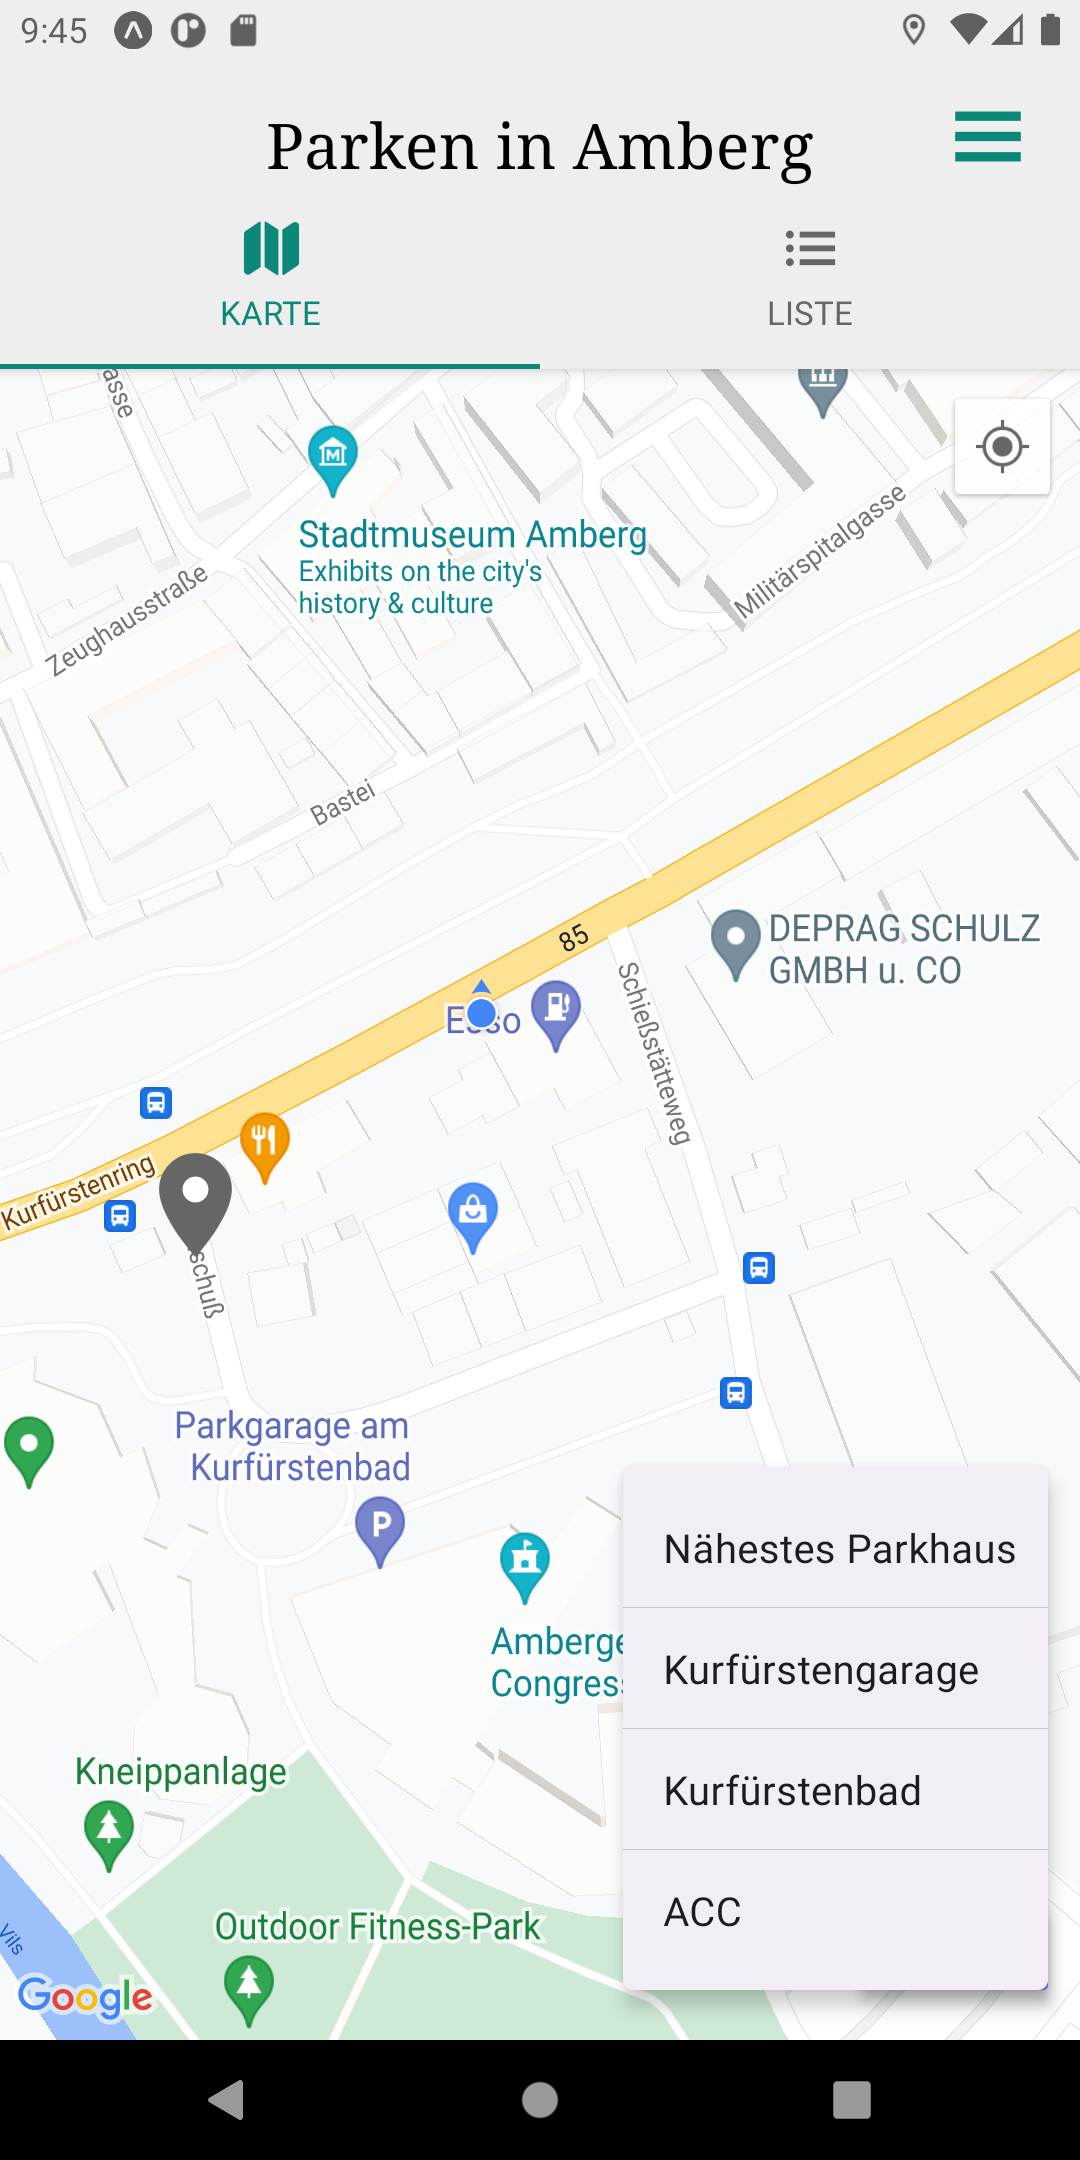
\includegraphics[scale=0.15]{img/geofence_navigation}
	\caption{Menü zur Navigation der Parkhäuser, in dessen Geofences sich der Nutzer befindet}
	\label{fig:geofence_navigation}
\end{wrapfigure}
Der zweite Effekt des Drückens dieses Knopfes wird automatisch ausgeführt, wenn sich der Nutzer in einem oder mehreren der Geofences befindet, also der Abstand zwischen der Position des Nutzers und einem Parkhaus unter 200 Meter ist. Dann erscheint ein weiteres Menü von react-native-paper, wie in \autoref{fig:geofence_navigation} zu sehen ist. Hier werden nun mehrere Einträge angezeigt, aus denen der Nutzer wählen kann. Der erste Eintrag ist immer die Navigation zum nähesten Parkhaus. Durch Drücken dieses Eintrags findet derselbe Ablauf statt, wie oben beschrieben. Die weiteren Einträge sind die Namen der Parkhäuser, in deren Geofences der Nutzer sich befindet. Wenn einer dieser Einträge gedrückt wird, findet eine Navigation über die \verb|findCorrectGpxFile|-Funktion statt, die exakt zu diesem Parkhaus navigiert. Dabei wird die Navigation zu einem bestimmten Parkhaus verwendet, die in \autoref{chap:5} beschrieben ist. Da der Nutzer maximal einen Abstand von 200 Metern zu jedem dieser Einträge besitzen kann, da er ja sonst nicht in den Geofences wäre, ist die Wahrscheinlichkeit hoch, dass eine interne Navigation möglich ist, denn der Nutzer befindet sich dann wahrscheinlich auf dem Altstadtring. Wenn eine interne Navigation gestartet wird, erscheint wieder der ,,Abbrechen''-Knopf, um diese zu beenden.

Damit sind alle Funktionen und Komponenten der App beschrieben. Im Folgenden wird ein Ausblick gegeben, welche Schritte sinnvoll wären, um die App zu verbessern und eine Zusammenfassung der Entwicklung.

%\begin{itemize}
%	\item Tab-Navigation zwischen Liste und Karte
%	\item Navigations-Knopf unten rechts mit Auswahl, ob nächstes Parkhaus oder Parkhaus in Geofence
%	\item Genaue Preisdaten als Tabelle in Details zu Parkhaus
%	\item Navigation von überall in der App zu jedem Parkhaus möglich
%\end{itemize}